\documentclass[12pt]{article}
\usepackage{pdfpages}
\usepackage{setspace}
\usepackage[dutch]{babel}

% Importeer configuratie-instellingen
\newcommand{\folder}{C:/Users/Admin/Documents/Github/Statistiek}
\RequirePackage{\folder/LaTeX/styles/exam_config}
\RequirePackage{\folder/LaTeX/styles/statistics-macros}

\renewcommand{\baselinestretch}{1.5}
% Begin van het document
\begin{document}

% FMW-specifiek titelblad voordat het examen begint
\includepdf[pages=-]{../../Python/FMW_titelblad_20261106.pdf}
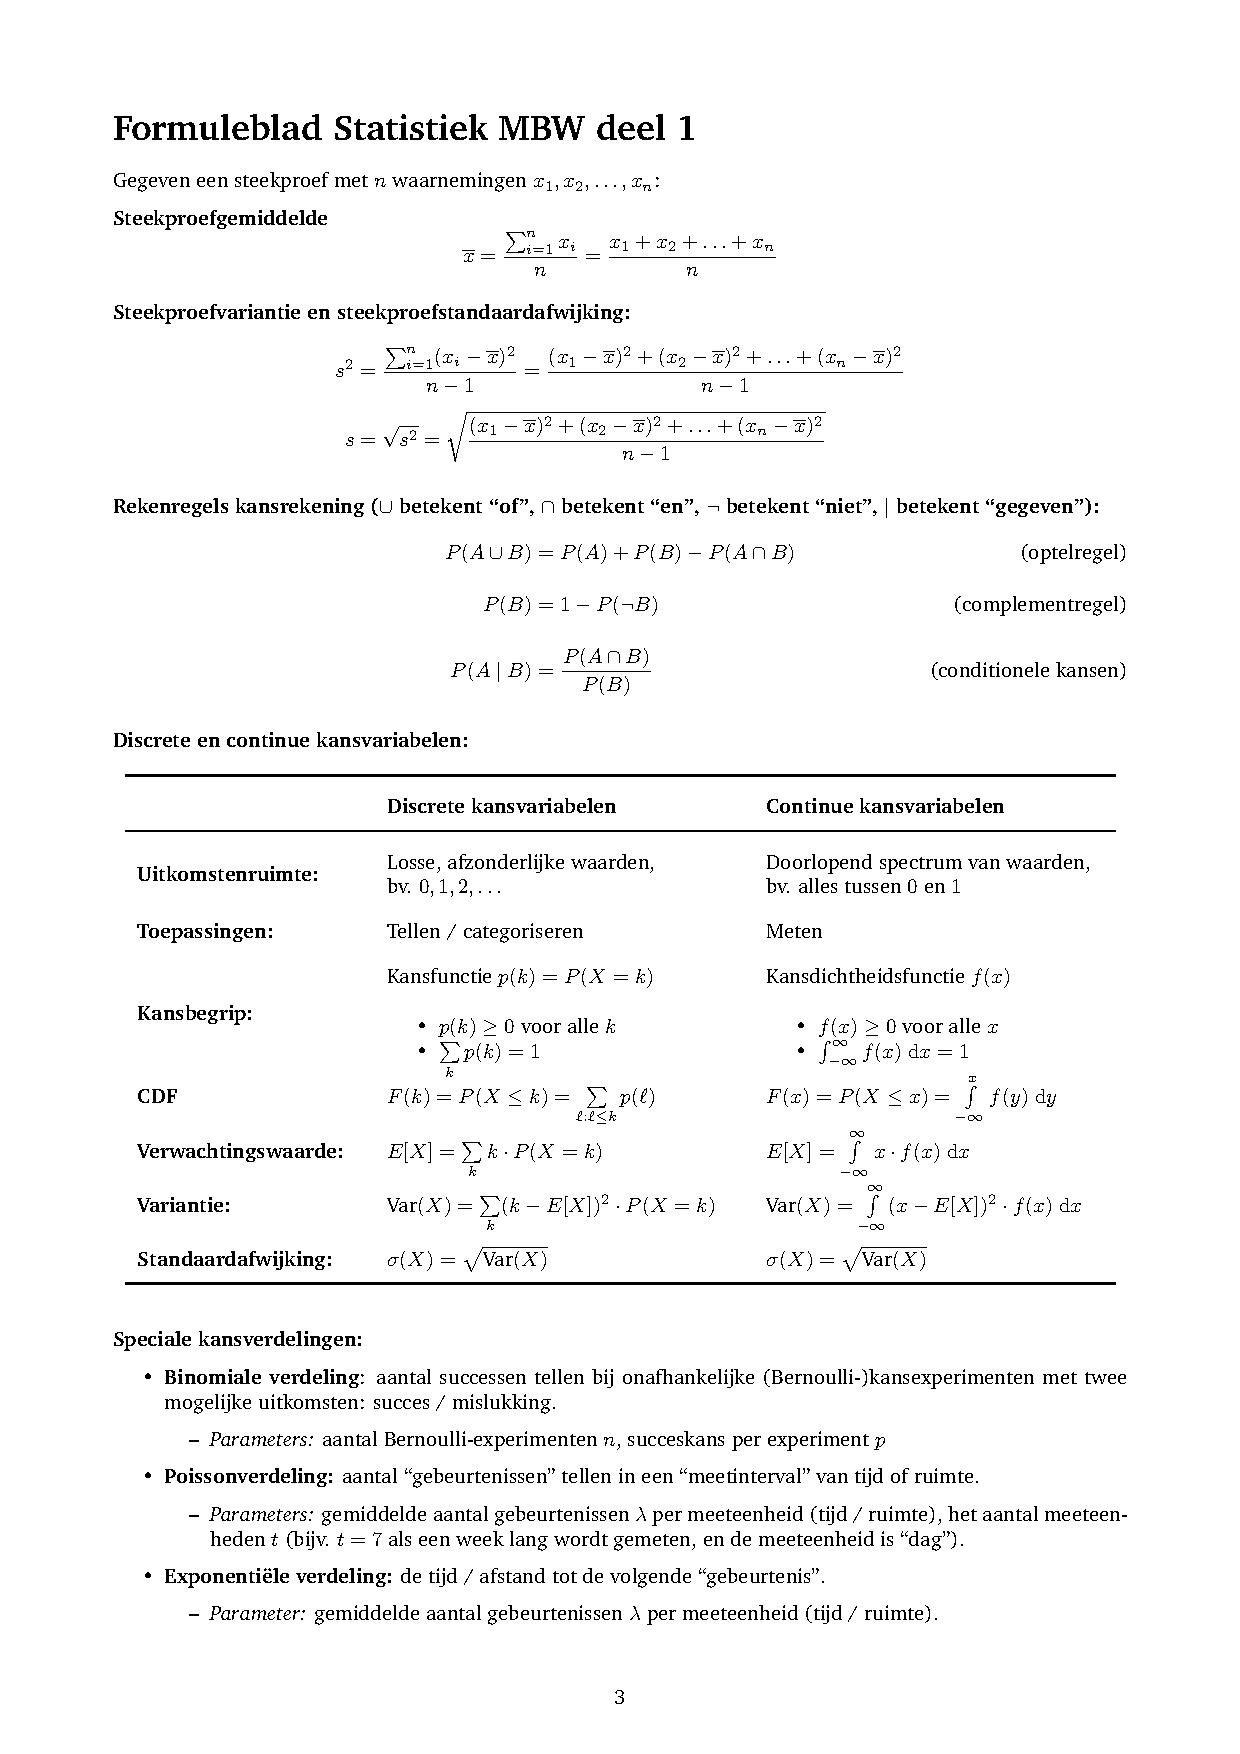
\includepdf[pages=-]{../../LaTeX/formulebladen/Formuleblad_STA2_2026.pdf}

% Include questions from external files
\begin{question}{18}{
    Het Commando Landstrijdkrachten (CLAS) test een nieuw type accu voor draagbare communicatiemiddelen.
    De fabrikant claimt een gemiddelde gebruiksduur van $\mu_0 = 36$ uur per volledig opgeladen accu.
    Uit eerdere productreeksen is bekend dat de gebruiksduur normaal verdeeld is met een \emph{bekende} standaardafwijking van $3.0$ uur.
    Een testpartij van $n = 25$ accu's geeft een steekproefgemiddelde van $34.6$ uur.
}

    \subquestion{6}{
        Bereken een tweezijdig \SI{96}{\percent}-betrouwbaarheidsinterval voor de gemiddelde gebruiksduur $\mu$ op basis van de gegeven steekproefdata.
        Rond de grenzen af op één decimaal, zodanig dat de betrouwbaarheid gewaarborgd blijft.
        Is er reden om aan te nemen dat de gemiddelde gebruiksduur significant afwijkt van $36$ uur?
    }

    \solution{
        In de vraag is gegeven dat $\mu_0 = 36$ uur, het steekproefgemiddelde
        $\samplemeanx = 34.6$ uur, de populatiestandaardafwijking
        $\sigma = 3.0$ uur en de steekproefgrootte $n = 25$.

        De gebruiksduur $X$ van een willekeurige accu is normaal verdeeld met $\mu = \text{ ?}$ en $\sigma = 3.0$. 
        We willen een betrouwbaarheidsinterval voor de onbekende $\mu$ berekenen op basis van de steekproefgegevens. 
        
        Omdat de standaardafwijking $\sigma$ bekend is, mogen we een betrouwbaarheidsinterval bepalen met behulp van de normale verdeling.\rubric{1}
        
        Verder is $\alpha = 0.04$, omdat we een \SI{96}{\percent}-betrouwbaarheidsinterval willen berekenen.
        De bijbehorende $z$-waarde is gelijk aan
        \[
            z_{\alpha/2} = \invnorm(\opp=1-\frac{\alpha}{2}=0.98, \mu=0, \sigma=1) \approx 2.0537.\rubric{1}
        \]
        Het \SI{96}{\percent}-betrouwbaarheidsinterval wordt dan gegeven door
        \begin{align*}
            &\phantom{=}[\samplemeanx - z_{\alpha/2} \cdot \frac{ \sigma }{ \sqrt{ n } }, \samplemeanx + z_{\alpha/2} \cdot \frac{ \sigma }{ \sqrt{ n } }] \\
            &= [34.6 - 2.0537 \cdot \frac{ 3.0 }{ \sqrt{ 25 } }, 34.6 + 2.0537 \cdot \frac{ 3.0 }{ \sqrt{ 25 } }] \\
            &= [33.3678, 35.8322].\rubric{2}
        \end{align*}
        Om de betrouwbaarheid te waarborgen, moeten we het interval naar buiten afronden, 
        oftewel op één decimaal afgerond krijgen we een interval van $[33.3, 35.9]$ uur. \rubric{1}

        Omdat de oorspronkelijke waarde $\mu_0 = 36$ uur niet in het betrouwbaarheidsinterval ligt, is er voldoende reden om aan te nemen dat de gemiddelde gebruiksduur significant afwijkt van $36$ uur.
        Specifiek is er voldoende reden om aan te nemen dat de gemiddelde gebruiksduur significant lager is dan $36$ uur.\rubric{1}
    }

    \subquestion{4}{
        De fabrikant wil de gemiddelde gebruiksduur nauwkeuriger schatten, namelijk met een maximale afwijking van $\pm 0.5$ uur bij \SI{96}{\percent} betrouwbaarheid.
        Wat is de minimaal benodigde steekproefomvang $n$ om met deze nauwkeurigheid te kunnen schatten?
    }

    \solution{
        Omdat de populatiestandaardafwijking $\sigma = 3.0$ bekend is, kunnen we gebruik maken van de volgende formule
        voor de minimaal benodigde steekproefomvang $n$ om een \SI{96}{\percent}-betrouwbaarheidsinterval te bepalen met afwijking $a = 0.5$:
        \[
            n \geq \left( \frac{z_{\alpha/2} \cdot \sigma}{a} \right)^2. \rubric{1}
        \]
        Invullen van de gegeven informatie geeft:
        \begin{align*}
            n   &\geq \left( \frac{z_{\alpha/2} \cdot \sigma}{a} \right)^2 \\
                &= \left( \frac{2.0537 \cdot 3.0}{0.5} \right)^2 \\
                &\approx 151.8438. \rubric{1}
        \end{align*}
        Aangezien de steekproefomvang $n$ een geheel getal moet zijn en we met grotere $n$ steeds nauwkeuriger kunnen schatten met dezelfde betrouwbaarheid,
        moeten we dit antwoord afronden naar boven. \rubric{1}

        We hebben dus minstens $n = 152$ accu's nodig. \rubric{1}
    }

    \subquestion{8}{
        CLAS is niet tevreden over de kwaliteit van de accu's van deze leverancier, en doet daarom een bestelling bij een tweede leverancier.
        Er worden voor een test $n = 36$ accu's bij deze nieuwe leverancier besteld.
        Van deze steekproef wordt bepaald dat de gemiddelde gebruiksduur gelijk is aan $35.5$ uur.
        Neem aan dat we nog steeds mogen werken met dezelfde \emph{bekende} standaardafwijking van $3.0$ uur. 
        
        CLAS is vooral geïnteresseerd in de vraag of de accu's gemiddeld \emph{korter} meegaan dan $36$ uur.
        Voer hiervoor een geschikte hypothesetoets uit met behulp van het kritieke gebied.
        Gebruik een significantieniveau $\alpha = 0.04$.
    }

    \solution{
        \subsubsection*{Stap 1: formuleer de nulhypothese $H_0$ en de alternatieve hypothese $H_1$.}
        Bij een toets of het gemiddelde $\mu$ van een normale verdeling kleiner is dan $\mu_0=36$ gebruiken we de volgende hypotheses
        \begin{align*}
            H_0: \quad \mu \geq 36\\
            H_1: \quad \mu < 36 \rubric{1}
        \end{align*}

        \subsubsection*{Stap 2: bepaal het significantieniveau $\alpha$.}
        Er is in de vraag gegeven dat we mogen werken met een significantieniveau $\alpha=0.04$.
        
        \subsubsection*{Stap 3: verzamel data voor het berekenen van de toetsingsgrootheid.}
        Ook is er in de vraag al steekproefdata verzameld voor de populatie accu's van de tweede leverancier, namelijk
        $\overline{x} = 35.5$. 

        \subsubsection*{Stap 4: bereken de toetsingsgrootheid.}
        De theoretische toetsingsgrootheid (hoofdletter!) bij een $z$-toets ($\sigma = 3.0$ is bekend!) is gelijk aan het steekproefgemiddelde $\overline{X}$. \rubric{1}
    
        Deze toetsingsgrootheid volgt onder $H_0$ een normale verdeling met $\mu = 36$ en $\sigma = \frac{3.0}{\sqrt{36}} = 0.5$. \rubric{1}
        
        De geobserveerde toetsingsgrootheid (kleine letter!) is gelijk aan $\overline{x} = 35.5$.
        
        \subsubsection*{Stap 5: bepaal de toetsuitslag (met behulp van het kritieke gebied).}

        Aangezien we een linkszijdige toets uitvoeren, is het kritieke gebied van de vorm $(-\infty, g)$, waarbij
        \[
            g = \invnorm(\opp=\alpha=0.04, \mu=36, \sigma=0.5) \approx 35.1247.
        \]        
        Het kritieke gebied is dus gelijk aan $(-\infty, 35.1247)$. \rubric{3}

        De geobserveerde toetsingsgrootheid $x = 35.5$ ligt niet in het kritieke gebied,
        dus we besluiten om $H_0$ niet te verwerpen.\rubric{1}

        \subsubsection*{Stap 6: vertaal de toetsuitslag terug naar de originele context van het probleem.}
        Er is onvoldoende reden om op basis van deze steekproef aan te nemen dat de gemiddelde gebruiksduur $\mu$
        van accu's van de tweede leverancier significant kleiner dan $36$ uur is.\rubric{1}
        \begin{center}
            \resizebox{0.9\textwidth}{!}{
                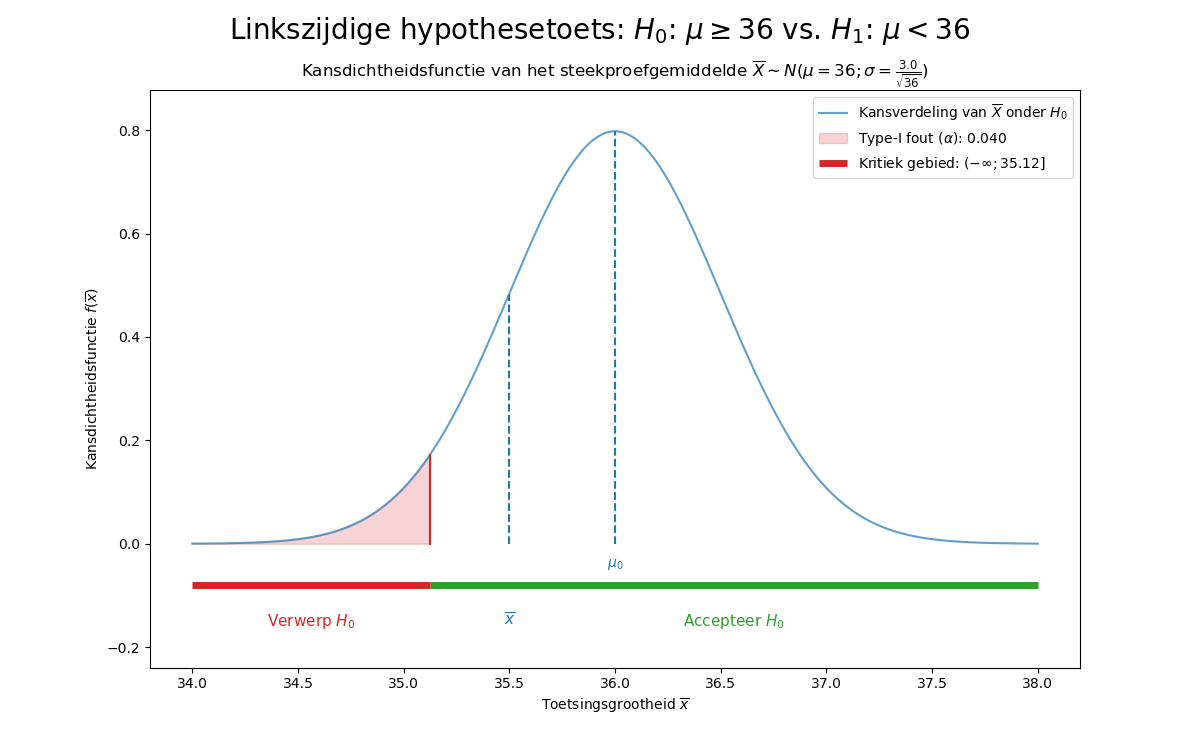
\includegraphics{../../LaTeX/figures/exam20261106_q1c.png}
            }
        \end{center}
    }

\end{question}

\begin{question}{28}{
    Binnen Defensie wordt een phishing-oefening gedaan, waarbij naar een willekeurig geselecteerde steekproef van $300$ werknemers 
    een nep-e-mail gestuurd wordt met een verdachte link.
    Per medewerker wordt bijgehouden hoe hij/zij op de e-mail heeft gereageerd en of de medewerker een cyber-awarenesstraining heeft gevolgd.
    \par\medskip
    \begin{center}
        \renewcommand{\arraystretch}{1}
        \begin{tabular}{m{0.28\textwidth}cccc}
            \toprule
                & \textbf{Meldt e-mail} & \textbf{Negeert e-mail} & \textbf{Klikt op link} & \textbf{Totaal} \\
            \midrule
                \textbf{Cybertraining} & $72$ & $55$ & $30$ & $157$  \\
                \textbf{Geen cybertraining} & $62$ & $37$ & $44$ & $143$ \\
            \midrule
                \textbf{Totaal} & $134$ & $92$ & $74$ & $300$ \\
            \bottomrule
        \end{tabular}
    \end{center}
    De Defensiestaf wil graag weten of het gevolgd hebben van cyber-awarenesstraining daadwerkelijk invloed heeft gehad op het adequaat reageren op de nep-e-mail.
}

    \subquestion{3}{
        Wat voor type hypothesetoets zou geschikt zijn om dit te kunnen toetsen?
        Formuleer de bijbehorende nulhypothese $H_0$ en de alternatieve hypothese $H_1$ voor deze toets.
    }

    \solution{
        Om te bepalen of er een statistisch significant effect is van het al dan niet volgen van de cyber-awarenesstraining voor het adequaat reageren
        op een nep-e-mail, dienen we een chikwadraattoets voor onafhankelijkheid uit te voeren. \rubric{1}
        De nulhypothese $H_0$ en de alternatieve hypothesetoets $H_1$ kunnen dan als volgt worden geformuleerd:
        \begin{itemize}
            \item[$H_0$:] er is sprake van onafhankelijkheid tussen het wel/niet volgen van de training en het type reactie op de nep-e-mail.\rubric{1}
            \item[$H_1$:] er is GEEN sprake van onafhankelijkheid tussen het wel/niet volgen van de training en het type reactie op de nep-e-mail. \rubric{1}
        \end{itemize}
    }

    \subquestion{8}{
        Wat is de theoretische toetsingsgrootheid van deze hypothesetoets?
        Bereken de geobserveerde toetsingsgrootheid met behulp van de data in bovenstaande tabel.
    }
    \solution{
        De (theoretische) toetsingsgrootheid voor een chikwadraattoets voor onafhankelijkheid is gelijk aan
        \[
            X^2 = \sum_{i,j} \frac{(O_{ij}-E_{ij})^2}{E_{ij}}.\rubric{1}
        \]    
        Voordat we de toetsingsgrootheid kunnen berekenen, moeten we dus de verwachte frequenties $E_{ij}$ bepalen.
        Dit doen we aan de hand van de volgende formule:
        \[
            E_{ij} = \frac{(\text{rijtotaal}_i) \cdot (\text{kolomtotaal}_j)}{\text{totaal}} \rubric{1}
        \]
        We berekenen de verwachte frequenties voor elke cel in de tabel:
        \par\medskip
        \begin{center}
            \renewcommand{\arraystretch}{1}
            \begin{tabular}{m{0.28\textwidth}|ccc|c}
                \toprule
                    & \textbf{Meldt e-mail} & \textbf{Negeert e-mail} & \textbf{Klikt op link} & \textbf{Totaal} \\
                \midrule
                \textbf{Cybertraining} & $70.1267$ & $48.1467$ & $38.7267$ & $157$ \\ 
            \textbf{Geen cybertraining} & $63.8733$ & $43.8533$ & $35.2733$ & $143$ \\ 
                \midrule
                    \textbf{Totaal} & $134$ & $92$ & $74$ & $300$ \rubric{3} \\
                \bottomrule
            \end{tabular}
        \end{center}
        \par\medskip
        Vervolgens berekenen we de geobserveerde toetsingsgrootheid $\chi^2$ als volgt:
        \begin{align*}
            \chi^2 &= \frac{(o_{1, 1} - e_{1,1})^2}{e_{1, 1}} + \frac{(o_{1, 2} - e_{1,2})^2}{e_{1, 2}} + \ldots + \frac{(o_{2, 3} - e_{2,3})^2}{e_{2, 3}} \\
                    &= \frac{(72 - 70.1267)^2}{70.1267} + \frac{(55 - 48.1467)^2}{48.1467} + \ldots + \frac{(44 - 35.2733)^2}{35.2733} \\
                    &\approx 6.2770. \rubric{3}
        \end{align*}
    }

    \subquestion{5}{
        Wat is de kansverdeling van de theoretische toetsingsgrootheid onder $H_0$? 
        Bereken met deze kansverdeling de $p$-waarde behorende bij de geobserveerde toetsingsgrootheid.
    }
    \solution{
        De theoretische toetsingsgrootheid $X^2$ volgt onder de nulhypothese een chikwadraatverdeling met $\df = (\#\text{rijen}-1)\cdot(\#\text{kolommen}-1) = (2-1)\cdot(3-1) = 2$ vrijheidsgraden. \rubric{2}
        De $p$-waarde is de kans dat de theoretische toetsingsgrootheid $X^2$ een \enquote{nog extremere} uitkomst aanneemt dan de geobserveerde toetsingsgrootheid $\chi^2$. \rubric{1}
        
        Aangezien een chikwadraattoets voor onafhankelijkheid altijd rechtszijdig is, is de $p$-waarde gelijk aan
        \begin{align*}
            p   &= P(\chi^2 > 6.2770) \\ 
                &= \chi^2\text{cdf}(\lb=6.2770; \ub=10^{99}, \df=2) \\
                &\approx 0.0433.  \rubric{2} 
        \end{align*}

        \begin{center}
            \resizebox{0.9\textwidth}{!}{
                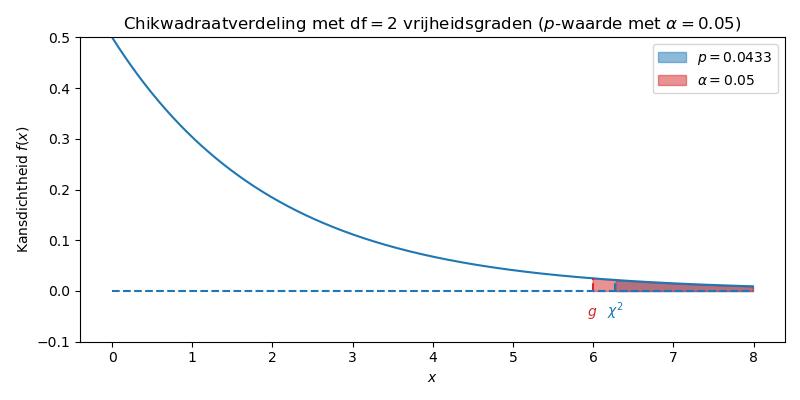
\includegraphics{exam20261106-chi2-pvalue.png} 
            }
        \end{center}
    }

    \subquestion{4}{
        Bepaal de toetsuitslag op basis van de berekende $p$-waarde en vertaal deze terug naar de originele probleemcontext.
        Gebruik hiervoor een significantieniveau $\alpha = 0.05$.
        Geef een verklaring voor de toetsuitslag met behulp van de tabel van geobserveerde en verwachte frequenties.
    }
    \solution{
        Aangezien de $p$-waarde $p \approx 0.0433$ strikt kleiner is dan het significantieniveau $\alpha = 0.05$,
        besluiten we om de nulhypothese $H_0$ te verwerpen. \rubric{1}

        Er is voldoende reden om aan te nemen dat het gevolgd hebben van een cyber-awarenesstraining
        significant effect heeft op de manier waarop op een nep-e-mail wordt gereageerd. \rubric{1}
        
        Als we kijken naar de tabellen van geobserveerde en verwachte frequenties,
        dan zien we dat voor de cellen met kenmerk \enquote{klikt op e-mail} de groep die geen training gevolgd heeft vaker dan verwacht (onder onafhankelijkheid) op de link heeft geklikt,
        terwijl dit bij de groep die wel training gevolgd heeft andersom is.\rubric{2}
    }
    
    \subquestion{8}{
        De commandant van de cybereenheid die deze nep-e-mail heeft verspreid beweert dat \SI{20}{\percent} van de Defensiemedewerkers op de link klikt.
        Bereken met de Clopper-Pearson methode een \SI{95}{\percent}-betrouwbaarheidsinterval voor de kans $p$ dat een willekeurige medewerker op de link klikt.
        Wat kunnen we concluderen over de claim van de commandant?
    }

    \solution{
        Van de $300$ medewerkers naar wie de link is verstuurd, hebben $30+44 = 74$ medewerkers op de link gedrukt (steekproef!).\rubric{1}
        Ervan uitgaande dat iedere medewerker onafhankelijk van elkaar wel of niet op de klik drukt, is het aantal medewerkers dat op
        de link drukt een binomiale kansvariabele $X$ met $n = 300$ en een onbekende succeskans $p = \text{ ?}$. \rubric{1}
        Op basis van deze aantallen gaan we een betrouwbaarheidsinterval bepalen voor de kans $p$ dat een willekeurige medewerker
        op de link drukt (populatieparameter!).
        Omdat de gewenste betrouwbaarheid \SI{95}{\percent} is, geldt dat $\alpha = 0.05$.

        De Clopper-Pearson methode werkt als volgt:
        \begin{enumerate}
            \item Bepaal de minimale succeskans $p_1$ waarvoor de uitkomst $k = 74$ niet extreem groot is, oftewel $P(X \geq 74) = 1 - P(X \leq 73) = \alpha/2 \geq 0.025$.
            Voer hiervoor in de \enquote{numerieke solver} van de grafische rekenmachine in:
            \begin{align*}
                E_1 &= 1 - \binomcdf(n=300, p_1=X, k=74) \\
                E_2 &= 0.025 
            \end{align*}
            De \enquote{numerieke solver} geeft een waarde van $p_1 \approx 0.1989$.
            \item Bepaal de maximale succeskans $p_2$ waarvoor de uitkomst $k = 74$ niet extreem klein is, oftewel $P(X \leq 74) = \alpha/2 \geq 0.025$.
            Voer hiervoor in de \enquote{numerieke solver} van de grafische rekenmachine in:
            \begin{align*}
                E_1 &= \binomcdf(n=300, p_1=X, k=74) \\
                E_2 &= 0.025 
            \end{align*}
            De \enquote{numerieke solver} geeft een waarde van $p_2 \approx 0.2995$.
        \end{enumerate}
        We vinden het Clopper-Pearson interval door de twee gevonden waarden als grenzen te nemen,
        oftewel het \SI{95}{\percent}-betrouwbaarheidsinterval voor de kans $p$ dat een willekeurige medewerker op de link klikt
        is gelijk aan $[0.1989, 0.2995]$. \rubric{4}

        We zien dat de geclaimde succeskans $p = 0.20$ in het Clopper-Pearson interval ligt. \rubric{1}
        Deze geobserveerde steekproefresultaten geven dus onvoldoende reden om de claim van de commandant naast ons neer te leggen.\rubric{1}
    }
\end{question}
\begin{question}{30}{
    De Koninklijke Marine vergelijkt twee sonarsystemen, $A$ en $B$, op haar fregatten.
    Tegen hetzelfde type doel is de detectieafstand (in \si{\kilo\metre}) gemeten bij acht oefeningen met systeem $A$ en tien oefeningen met systeem $B$.
    Neem aan dat de afstanden normaal verdeeld zijn met onbekende gemiddelden $\mu_A$ en $\mu_B$ en standaardafwijkingen $\sigma_A$ en $\sigma_B$.

    \begin{center}
        \begin{tabular}{m{0.24\textwidth}|cccccccccccc}
            \toprule
                \textbf{Detectieafstanden $A$} & $18.2$ & $17.5$ & $18.8$ & $17.9$ & $18.4$ & $17.7$ & $18.1$ & $18.6$ &        &        \\
            \midrule
                \textbf{Detectieafstanden $B$} & $16.5$ & $19.4$ & $15.2$ & $18.8$ & $14.9$ & $17.6$ & $19.9$ & $16.1$ & $18.3$ & $15.8$ \\
            \bottomrule
        \end{tabular}
    \end{center}
    Je mag in deze vraag bij hypothesetoetsen gebruik maken van een significantieniveau $\alpha = 0.05$.
}

    \subquestion{6}{
        Bereken de steekproefgemiddelden en de steekproefvarianties van de detectieafstanden van beide sonarsystemen.
    }
    \solution{
    
        We berekenen het steekproefgemiddelde $\overline{x_A}$ voor de $n = 8$ detectieafstanden van sonarsysteem $A$ als volgt:
        \begin{align*}
            \overline{x_A} = \frac{a_1+a_2+\ldots+a_n}{n} = \frac{ 18.2 + 17.5 + \ldots + 18.6 }{ 8 } = 18.15.\rubric{1}
        \end{align*}
    
        We berekenen de steekproefvariantie $s_A^2$ als volgt:
        \begin{align*}
            s_A^2 &= \frac{ (a_1 - \overline{x_A})^2 + (a_2 - \overline{x_A})^2 + \ldots + (a_n - \overline{x_A})^2 }{ n - 1 } \\
                &= \frac{ (18.2 - 18.15)^2 + (17.5 - 18.15)^2 + \ldots + (18.6 - 18.15)^2 }{ 8 - 1 } \\
                &\approx 0.1971.\rubric{3}
        \end{align*}

        We berekenen het steekproefgemiddelde $\overline{x_B}$ voor de $m = 10$ detectieafstanden van sonarsysteem $A$ als volgt:
        \begin{align*}
            \overline{x_B} = \frac{b_1+b_2+\ldots+b_m}{m} = \frac{ 16.5 + 19.4 + \ldots + 15.8 }{ 10 } = 17.25.\rubric{1}
        \end{align*}
    

        We berekenen de steekproefvariantie $s_B^2$ als volgt:
        \begin{align*}
            s_B^2 &= \frac{ (b_1 - \overline{x_B})^2 + (b_2 - \overline{x_B})^2 + \ldots + (b_m - \overline{x_B})^2 }{ m - 1 } \\
                &= \frac{ (16.5 - 17.25)^2 + (19.4 - 17.25)^2 + \ldots + (15.8 - 17.25)^2 }{ 10 - 1 } \\ \rubric{2}
                &\approx 3.2206.
        \end{align*}
    }

    \subquestion{10}{
        Voer een $F$-toets uit om te bepalen of de varianties in de detectieafstanden gelijk kunnen zijn voor beide sonarsystemen.
        Geef hierbij expliciet de stappen aan van het algemene stappenplan voor hypothesetoetsen.
        Bepaal de toetsuitslag op basis van het kritieke gebied.
    }
    \solution{
        \subsubsection*{Stap 1: formuleer de nulhypothese $H_0$ en de alternatieve hypothese $H_1$.}
        Bij een $F$-toets toetsen we of de varianties $\sigma_A^2$ en $\sigma_B^2$ gelijk zouden kunnen zijn, oftewel
        \begin{align*}
            H_0: \quad \sigma_A^2 = \sigma_B^2 \\
            H_1: \quad \sigma_A^2 \neq \sigma_B^2 \rubric{1}
        \end{align*}

        \subsubsection*{Stap 2: bepaal het significantieniveau $\alpha$.}
        Er is in de vraag gegeven dat we mogen werken met een significantieniveau $\alpha=0.05$.
        
        \subsubsection*{Stap 3: verzamel data voor het berekenen van de toetsingsgrootheid.}
        Ook zijn er in de vraag al steekproefdata verzameld voor beide populaties. 
        Op basis van deze steekproefdata hebben we in vraag (a) bepaald dat:
        
        \begin{center}
            \begin{tabular}{C{.3\textwidth} C{.3\textwidth} C{.3\textwidth}}
                $\overline{x_A} = 18.15$ & $s_A^2 \approx 0.1971$ & $n = 8$ \\
                $\overline{x_B} = 17.25$ & $s_B^2 \approx 3.2206$ & $m = 10$
            \end{tabular}
        \end{center}

        \subsubsection*{Stap 4: bereken de toetsingsgrootheid.}
        De theoretische toetsingsgrootheid (hoofdletter!) bij een $F$-toets is gelijk aan
        \[
            F = \frac{S_A^2}{S_B^2}, \rubric{1}
        \]
        en volgt onder $H_0$ een $F$-verdeling met $\dfn = n-1 = 7$ en $\dfd = m-1 = 9$ vrijheidsgraden. \rubric{1}

        De geobserveerde toetsingsgrootheid (kleine letter!) is gelijk aan
        \[
            f = \frac{s_A^2}{s_B^2} = \frac{0.1971}{3.2206} \approx 0.0612. \rubric{1}
        \]
        
        \subsubsection*{Stap 5: bepaal de toetsuitslag (met behulp van het kritieke gebied).}

        Een $F$-toets voor gelijke varianties is altijd tweezijdig, oftewel het kritieke gebied is van de vorm $(0, g_1)$ en $(g_2, \infty)$, waarbij de grenswaarden $g_1$ en $g_2$ als volgt kunnen worden berekend:
        \begin{enumerate}
            \item Bepaal de grenswaarde $g_1$ waarvoor geldt dat $P(F \leq g_1) = \alpha/2 = 0.025$.
            Voer hiervoor in de \enquote{numerieke solver} van de grafische rekenmachine in:
            \begin{align*}
                E_1 &= \fcdf(\lb=0, \ub=X, \df_1=7, \df_2=9) \\
                E_2 &= 0.025
            \end{align*}
            De \enquote{numerieke solver} geeft een waarde van $g_1 \approx 0.2073$.
            \item Bepaal de grenswaarde $g_2$ waarvoor geldt dat $P(F \geq g_2) = \alpha/2 = 0.025$.
            Voer hiervoor in de \enquote{numerieke solver} van de grafische rekenmachine in:
            \begin{align*}
                E_1 &= \fcdf(\lb=X, \ub=\GRinfinity, \df_1=7, \df_2=9) \\
                E_2 &= 0.025
            \end{align*}
            De \enquote{numerieke solver} geeft een waarde van $g_2 \approx 4.1970$.
        \end{enumerate}
        
        Het kritieke gebied is dus gelijk aan $(0, 0.2073)$ en $(4.1970, \infty)$. \rubric{4}

        De geobserveerde toetsingsgrootheid $f \approx 0.0612$ ligt in het kritieke gebied, dus we besluiten om $H_0$ te verwerpen.\rubric{1}

        \subsubsection*{Stap 6: vertaal de toetsuitslag terug naar de originele context van het probleem.}
        Er is voldoende reden om op basis van deze steekproeven de aanname van gelijke varianties (van de detectieafstanden van beide sonarsystemen) te verwerpen, 
        oftewel we gaan er nu van uit dat $\sigma_X^2 \neq \sigma_Y^2$. \rubric{1}
    }

    \subquestion{10}{
        Bepaal met behulp van een geschikte $t$-toets of de gemiddelde detectieafstand significant groter is voor sonarsysteem $A$.
        Geef hierbij expliciet de stappen aan van het algemene stappenplan voor hypothesetoetsen.
        Bepaal hierbij de toetsuitslag met behulp van de $p$-waarde.
    }
    \solution{
        \subsubsection*{Stap 1: formuleer de nulhypothese $H_0$ en de alternatieve hypothese $H_1$.}
        We gaan toetsen of de gemiddelde detectieafstanden $\mu_A$ significant groter is dan $\mu_B$.
        De hypothesen zijn daarom als volgt:
        \begin{align*}
            H_0: &\quad \mu_A \leq  \mu_B \text{ (niet significant grotere gemiddelde voor $A$) } \\
            H_1: &\quad \mu_A > \mu_B \text{ (wel significant grotere gemiddelde voor $A$) } \rubric{2}
        \end{align*}

        \subsubsection*{Stap 2: bepaal het significantieniveau $\alpha$.}
        Er is opnieuw gegeven dat we mogen werken met een significantieniveau $\alpha=0.05$.
        
        \subsubsection*{Stap 3: verzamel data voor het berekenen van de toetsingsgrootheid}
        Ook zijn er in de vraag al steekproefdata verzameld voor beide populaties. 
        Op basis van deze steekproefdata hebben we in vraag (a) bepaald dat:
        
        \begin{center}
            \begin{tabular}{C{.3\textwidth} C{.3\textwidth} C{.3\textwidth}}
                $\overline{x_A} = 18.15$ & $s_A^2 \approx 0.1971$ & $n = 8$ \\
                $\overline{x_B} = 17.25$ & $s_B^2 \approx 3.2206$ & $m = 10$
            \end{tabular}
        \end{center}

        \subsubsection*{Stap 4: bereken de toetsingsgrootheid.}
        Op basis van ons antwoord bij vraag (b) mogen we aannemen dat de varianties ongelijk zijn, oftewel $\sigma_X^2 \neq \sigma_Y^2$.
        De theoretische toetsingsgrootheid (hoofdletter!) bij een $t$-toets met twee steekproeven (met ongelijke varianties) is gelijk aan
        \[
            T = \frac{(\overline{X_A} - \overline{X_B}) - (\mu_A - \mu_B)}{\sqrt{\frac{S_A^2}{n} + \frac{S_B^2}{m}}}, \rubric{1}
        \]
        en volgt onder $H_0$ een $t$-verdeling met $\df=\min(n-1,m-1)=7$ vrijheidsgraden. \rubric{1}

        De geobserveerde toetsingsgrootheid (kleine letter!) is gelijk aan
        \begin{align*}
            t   &= \frac{(\overline{x_A}-\overline{x_B}) - (\mu_A - \mu_B)}{\sqrt{\frac{s_A^2}{n} + \frac{s_B^2}{m}}} \\
                &= \frac{(18.15 - 17.25) - 0}{\sqrt{\frac{0.1971}{8} + \frac{3.2206}{10}}} \\
                &\approx 1.5285. \rubric{2}
        \end{align*}

        \subsubsection*{Stap 5: bepaal de toetsuitslag (met behulp van de $p$-waarde).}
        Omdat we rechtszijdig toetsen, is de $p$-waarde gelijk aan $P(T \geq t)$:
        Deze kans kunnen we met de $t$-verdeling bepalen, namelijk:
        \begin{align*}
            P(T \geq t) &= \tcdf(\lb = 1.5285, \ub=\GRinfinity, \df=7) \approx 0.0851.
        \end{align*}
        De $p$-waarde is dus gelijk aan $p \approx 0.0851$. \rubric{2}

        Aangezien de $p$-waarde strikt groter is dan $\alpha$, besluiten we om de nulhypothese niet te verwerpen.\rubric{1}
        
        \subsubsection*{Stap 6: vertaal de toetsuitslag terug naar de originele context van het probleem.}
        Er is op basis van deze steekproeven onvoldoende bewijs om aan te nemen dat de gemiddelde detectieafstand bij sonarsysteem $A$
        significant groter is dan bij sonarsysteem $B$. \rubric{1}    
        % \begin{center}
        %     \resizebox{0.9\textwidth}{!}{
        %         \includegraphics{exam20260724-two-sample-t-test-pvalue.png} 
        %     }
        % \end{center}
    }

    \subquestion{4}{
        Is er op basis van de twee toetsen een voorkeur voor één van de systemen aan te wijzen?
        Licht toe aan de hand van de gegeven steekproefdata en de conclusies van de twee toetsen.
    }
    \solution{
        Uit de $t$-toets is gebleken dat we niet kunnen zeggen dat de gemiddelden significant van elkaar verschillen.\rubric{1}

        Uit de $F$-toets echter bleek wel dat de spreiding significant verschilt; in het bijzonder geven de steekproefdata 
        aan dat de spreiding bij $B$ significant groter dan bij $A$.\rubric{1}

        Systeem $A$ is daardoor meer \enquote{voorspelbaar} qua performance, en $B$ levert soms zeer lage detectieafstanden (\SI{14.9}{\kilo\metre}),
        wat operationeel riskant is.\rubric{1}
        
        De voorkeur gaat dus uit naar $A$.\rubric{1}
    }
\end{question}
\begin{question}{24}{
    Bij de grenscontrole op Schiphol Airport onderzoekt de Koninklijke Marechaussee het verband tussen het aantal geopende controleloketten $X$ en de
    wachttijd $Y$ (in minuten) van reizigers naar een bestemming buiten het Schengengebied tijdens tien drukke ochtenden.
    {\par\bigskip
        \begin{center}
            \begin{tabular}{c|cccccccccc}
                \toprule
                    \textbf{$X$} & $2$ & $3$ & $4$ & $5$ & $6$ & $7$ & $8$ & $9$ & $10$ & $11$ \\
                \midrule
                    \textbf{$Y$} & $46.2$ & $41.3$ & $52.7$ & $36.1$ & $38.8$ & $41.6$ & $23.7$ & $11.0$ & $16.5$ & $14.2$ \\
                \bottomrule
            \end{tabular}
        \end{center}
    \par\bigskip}
}

    \subquestion{4}{
        Teken het spreidingsdiagram (scatter plot) op basis van de bovenstaande tabel.
        Geef hierbij ook duidelijk aan welke as welke variabele beschrijft.
    }
    \solution{
        De $x$-as duidt de onafhankelijke variabele $X$ uit, oftewel het aantal geopende controleloketten. \rubric{1}

        De $y$-as duidt de afhankelijke variabele $Y$ uit, oftewel de gemiddelde wachttijd van reizigers.\rubric{1}
        \begin{center}
            \resizebox{\textwidth}{!}{
                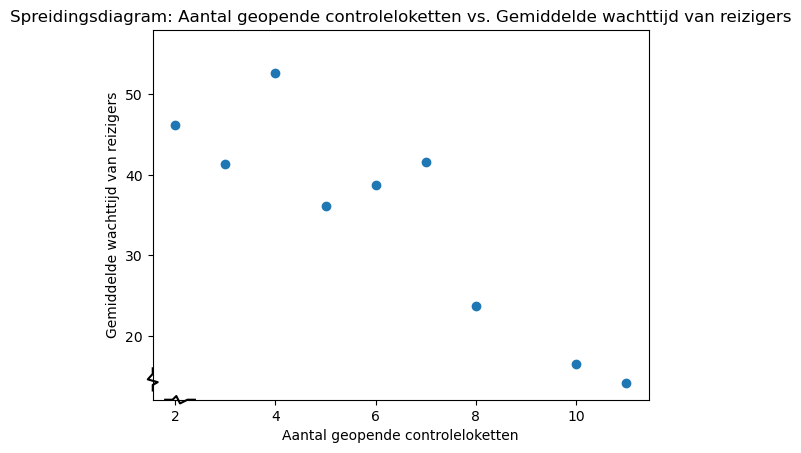
\includegraphics{exam20261106-scatterplot.png} \rubric{2}
            }
        \end{center}
    }

    \subquestion{7}{
        Bereken Pearson's correlatiecoëfficiënt $r(x,y)$ op basis van de data in de bovenstaande tabel.
        Wat zegt $r(x, y)$ over de relatie tussen het aantal geopende controleloketten en de wachttijd van reizigers?
    }
    \solution{
        We beginnen met het uitrekenen van Pearson's correlatiecoëfficiënt 
        \begin{align*}
            r(x, y)  &= \frac{ \overline{x \cdot y} - \overline{x} \cdot \overline{y} }{ \sqrt{ (\overline{x^2} - \overline{x}^2 ) \cdot (\overline{y^2} - \overline{y}^2) }}
        \end{align*}
        Hiervoor hebben we dus de waardes van $\overline{x}$, $\overline{y}$, $\overline{xy}$, $\overline{x^2}$ en $\overline{y^2}$ nodig.
        Deze bepalen we aan de hand van de volgende rekentabel:
        \begin{center}
            \begin{tabular}{ccccc}
                \toprule
                    $x$ & $y$ & $xy$ & $x^2$ & $y^2$ \\
                \midrule
    		        $2$  & $46.2$ & $92.4$  &   $4$ & $2134.44$ \\
                    $3$  & $41.3$ & $123.9$ &   $9$ & $1705.69$ \\
                    $4$  & $52.7$ & $210.8$ &  $16$ & $2777.29$ \\
                    $5$  & $36.1$ & $180.5$ &  $25$ & $1303.21$ \\
                    $6$  & $38.8$ & $232.8$ &  $36$ & $1505.44$ \\
                    $7$  & $41.6$ & $291.2$ &  $49$ & $1730.56$ \\
                    $8$  & $23.7$ & $189.6$ &  $64$ & $561.69$ \\
                    $9$  & $11.0$ & $99.0$  &  $81$ & $121.0$ \\
                    $10$ & $16.5$ & $165.0$ & $100$ & $272.25$ \\
                    $11$ & $14.2$ & $156.2$ & $121$ & $201.64$ \\
                \midrule
                    $\overline{x} = 6.5$ & $\overline{y} = 32.21$ & $\overline{xy} = 174.14$ & $\overline{x^2} = 50.5$ & $\overline{y^2} = 1231.321$ \rubric{3} \\ 
                \bottomrule
            \end{tabular}
        \end{center}
        \par\medskip
        De correlatiecoëfficiënt van Pearson is dus gelijk aan
        \begin{align*}
            r(x,y)  &= \frac{ \overline{x \cdot y} - \overline{x} \cdot \overline{y} }{ \sqrt{ (\overline{x^2} - \overline{x}^2) \cdot (\overline{y^2} - \overline{y}^2) } }\\
                    &= \frac{ 174.14 - 6.5 \cdot 32.21 }{ \sqrt{ (50.5 - 6.5^2) \cdot (1231.321 - 32.21^2) } } \\
                    &= \frac{-35.225}{39.9894} \\
                    &\approx -0.8809.
        \end{align*}
        De correlatiecoëfficiënt $r \approx -0.8809$ ligt ver van $0$ af en is negatief.
        Dit houdt in dat er een sterke negatieve lineaire (dalende) trend is. \rubric{1}
        Een groter aantal geopende controleloketten correleert sterk met een lagere wachttijd. \rubric{1}

        (Maximaal $2$ punten indien de student een positieve waarde heeft berekend voor $r(x, y)$ 
        en inziet dat dit niet rijmt met het spreidingsdiagram.
        $0$ punten indien de student dit besef niet laat zien in zijn/haar uitwerking.)
    }

    \subquestion{6}{
        Bereken de coëfficiënten $a$ en $b$ van de regressielijn $\hat{Y} = a + b \cdot X$.
        Bepaal aan de hand van de regressielijn een statistisch verantwoorde voorspelling voor de wachttijd van 
        reizigers op een willekeurige drukke dag wanneer er zes loketten geopend zijn.
    }
    \solution{
        Om de coëfficiënten $a$ en $b$ van de regressielijn te berekenen, gaan we de rekentabel van vraag (a) hergebruiken.
        Er volgt namelijk dat
        \begin{align*}
            b &= \frac{\overline{xy} - \overline{x} \cdot \overline{y}}{\overline{x^2} - (\overline{x})^2} \\
              &= \frac{174.1400 - 6.5 \cdot 32.21}{50.5 - (6.5)^2} \\
              &= \frac{-35.225}{8.25} \approx -4.2697 \\
            a &= \overline{y} - b \cdot \overline{x} \\
              &= 32.21 - -4.2697 \cdot 6.5 \\
              &\approx 59.9630.
        \end{align*}
        De formule van de regressielijn behorende bij deze steekproef is dus gelijk aan $Y = 59.9630-4.2697 \cdot X$. \rubric{1}
        Een statistisch verantwoorde voorspelling voor de wachttijd wanneer zes loketten zijn geopend
        vinden we door $x_0 = 6$ in te vullen:
        Dit geeft een waarde van $\hat{Y}_0 = 59.9630 - 4.2697 \cdot 6 \approx 34.3448$, oftewel 
        onze voorspelling zegt dat bij zes geopende loketten reizigers ruim $34$ minuten moeten wachten. \rubric{1} 

        (Geen punten indien $b > 0$ of extreem grote of kleine waarden voor $a$ en $b$ zonder besef dat dit niet kan kloppen. \\
        Maximaal $2$ punten indien de coëfficiënten dusdanige waarden hebben dat deze niet logischerwijs een passende lijn vormen door de steekproefdata.)
    }

    \subquestion{7}{
        Bereken een \SI{95}{\percent}-voorspellingsinterval voor de wachttijd van reizigers op een willekeurige dag waarop er zes loketten zijn geopend.
        Rond het interval af op gehele minuten zodat de betrouwbaarheid van het interval gewaarborgd blijft.
    }
    \solution{
        In opdracht (d) hebben we een puntschatting van $\hat{Y}_0 = 59.9630 - 4.2697 \cdot 6 \approx 34.3448$ bepaald.
        Daarnaast kunnen we de standaardafwijking $\sigma$ van de storingsterm $\varepsilon$ schatten:
        \begin{align*}
            s_{\varepsilon} &= \sqrt{ \frac{n}{n-2} \cdot \left( \overline{y^2} - a \cdot \overline{y} - b \cdot \overline{xy} \right) } \\ 
                               &= \sqrt{ \frac{10}{8} \cdot \left( 1231.321 - 59.9630 \cdot 32.21 - -4.2697 \cdot 174.14 \right) } \\ 
                               &\approx 7.3686.\rubric{2}
        \end{align*}

        Vervolgens kunnen we een puntschatting berekenen van de standaardafwijking van $Y$ voor gegeven $X = x_0$:
        \begin{align*}
            s_{f}   &= s_{\varepsilon} \cdot \sqrt{ 1 + \frac{1}{n} \cdot \left( 1 + \frac{(x_0 - \overline{x})^2}{\overline{x^2} - \overline{x}^2} \right) } \\
                    &= 7.3686 \cdot \sqrt{ 1 + \frac{1}{10} \cdot \left( 1 + \frac{(6 - 6.5)^2}{50.5 - 6.5^2} \right) } \\
                    &\approx 7.7389.\rubric{2}
        \end{align*}

        Omdat we de standaardafwijkingen geschat hebben en de storingstermen normaal verdeeld zijn, moeten we werken met de $t$-verdeling met $\df = n - 2 = 9$ vrijheidsgraden.
        De $t$-waarde die hoort bij een betrouwbaarheidsniveau $\alpha = 0.05$ is gelijk aan
        \[
            t = \invt(\opp = 1 - \alpha / 2, \df = n - 2) = \invt(\opp = 0.975, \df = 8) \approx 2.3060.\rubric{1}
        \]
        Het \SI{95}{\percent}-voorspellingsinterval voor $Y$ voor gegeven $X = 80$ kan dus worden beschreven door
        \begin{align*}
            &[\hat{Y}_0 - t \cdot s_{f}, \hat{Y}_0 - t \cdot s_{f}] \\
            &= [34.3448 - 2.3060 \cdot 7.7389; 34.3448 + 2.3060 \cdot 7.7389] \\ 
            &\approx [16.4990, 52.1907]. \rubric{1}
        \end{align*}
        
        Op een willekeurige drukke dag met zes geopende loketten moeten reizigers dus met \SI{95}{\percent} kans tussen
        $16$ en $53$ minuten wachten (dit is een heel groot interval, dus de nauwkeurigheid van de voorspelling is niet al te hoog;
        dit komt deels doordat de steekproefgrootte $n=10$ vrij klein is). \rubric{1}
    }
\end{question}

% Add more question files as needed
\end{document}